%!TEX program = xelatex
% Note: this template must be compiled with XeLaTeX rather than PDFLaTeX
% due to the custom fonts used. The line above should ensure this happens
% automatically, but if it doesn't, your LaTeX editor should have a simple toggle
% to switch to using XeLaTeX.

\documentclass[
  aspectratio=169, % Uncomment to use an aspect ratio of 16:9 (160 mm by 90 mm)
  %aspectratio=43, % Uncomment to use an aspect ratio of 4:3 (128mm by 96mm)
  t, % Top align all slide content by default
  onlytextwidth, % Typeset content in columns at text width
  10pt, % Default font size, use 10pt for the 16:9 aspect ratio and 8pt for the 4:3 aspect ratio
]{beamer}

\usepackage{../../ImperialTheme/beamer/beamerthemeImperial} % Use the Imperial theme

\def\imagefolder{../../ImperialTheme/beamer/Images}
\def\Rey{\text{Re}}
\title{Answering Jeff questions} % Presentation title to appear on the title slide and left footers

\subtitle{} % Presentation subtitle to appear on the title slide

\author{Víctor Ballester} % Author name(s) to appear on the title slide

\date{\today} % Presentation date to appear on the title slide and right footers

\begin{document}

\begingroup
\setbeamercolor{background canvas}{bg=ICLLightGrey} % Slide background color
\setbeamercolor{title page title}{fg=ICLBlue} % Title text color
\setbeamercolor{title page subtitle}{fg=ICLBlue} % Subtitle text color
\setbeamercolor{author}{fg=ICLBlue} % Author(s) text color
\setbeamercolor{date}{fg=ICLBlue} % Date text color
\setbeamertemplate{title page}[logo]{\imagefolder/ICL_Logo_Blue.pdf} % Imperial logo color, use 'ICL_Logo_White.pdf' for white and 'ICL_Logo_Blue.pdf' for blue
\frame[plain, s]{\titlepage} % Output the title page with no footer ('plain') and vertically distributed text ('s')
\endgroup

\begin{frame}
	\frametitle{Absolute instability going up to the upstream edge of the gap?}
	\begin{itemize}
		\item No. The colors are stressed, but they show that the absolute instability is localized near the downstream edge of the gap.
	\end{itemize}
	\centering
	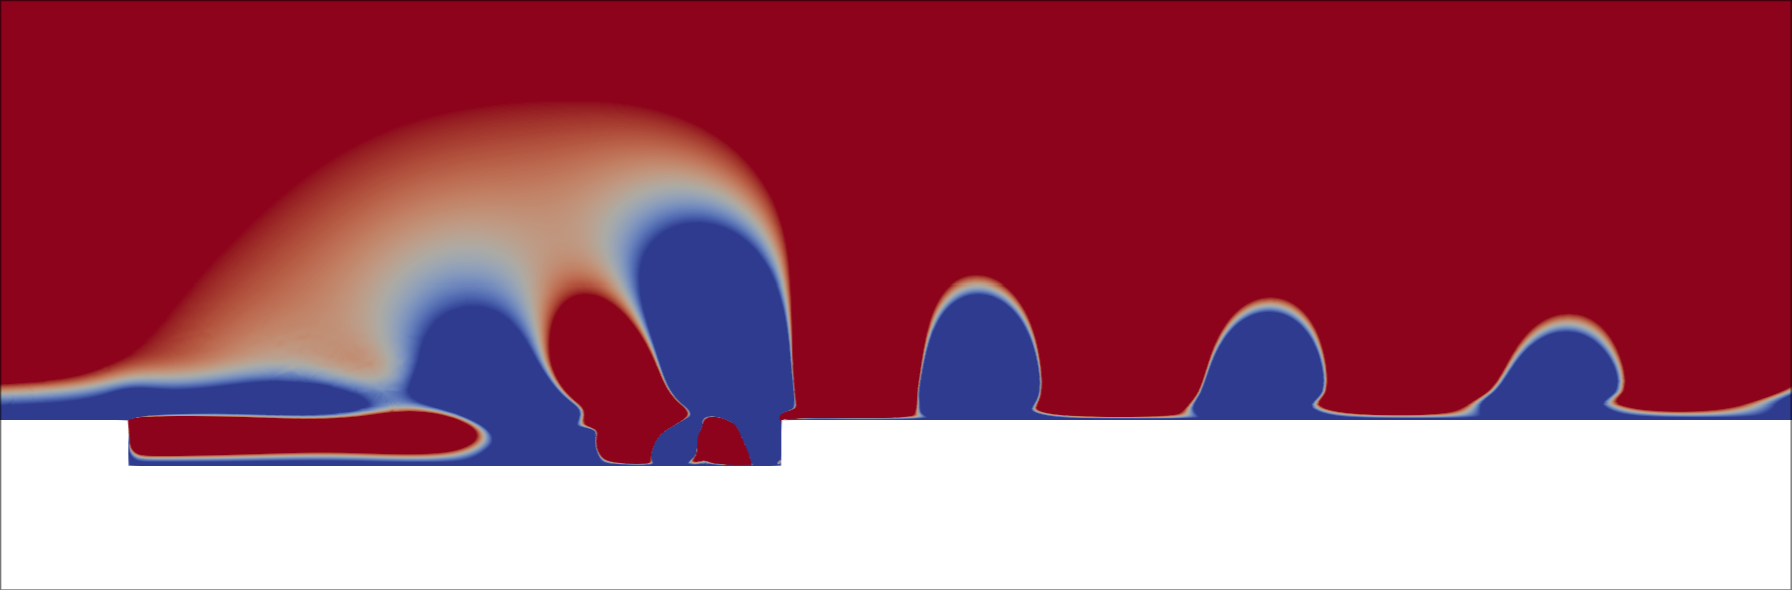
\includegraphics[width=0.75\linewidth]{Images/d2.25_w32.png}
	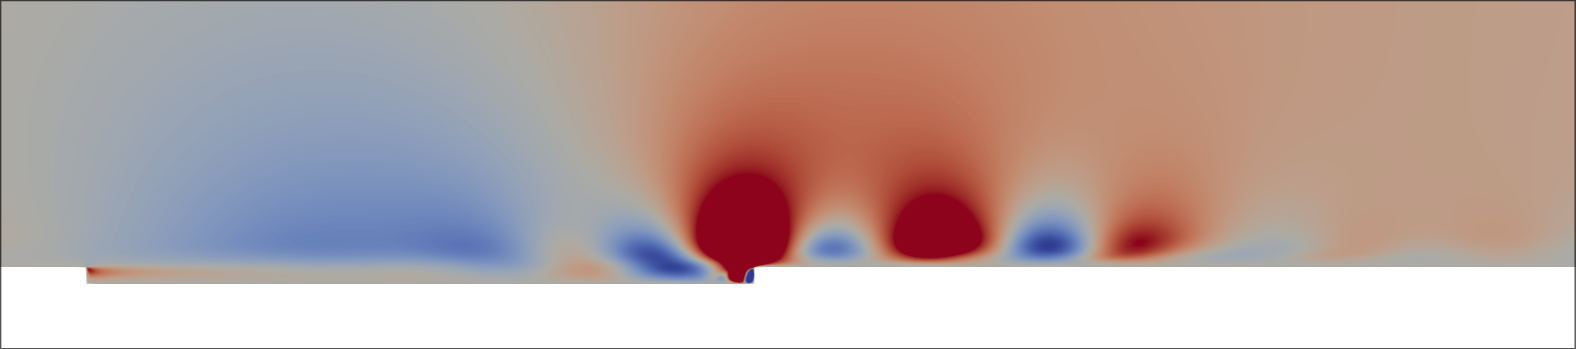
\includegraphics[width=0.75\linewidth]{Images/d1.5_w58.png}
\end{frame}
\begin{frame}
	\frametitle{Aboslute instability in the gap}
	SFD for $d=2.25$, $w=32$ 
	Most unstable mode (with positive growth rate):
\begin{columns}[T] % [T] ensures correct vertical alignment
		\begin{column}{0.48\linewidth} % Left column
			\centering
			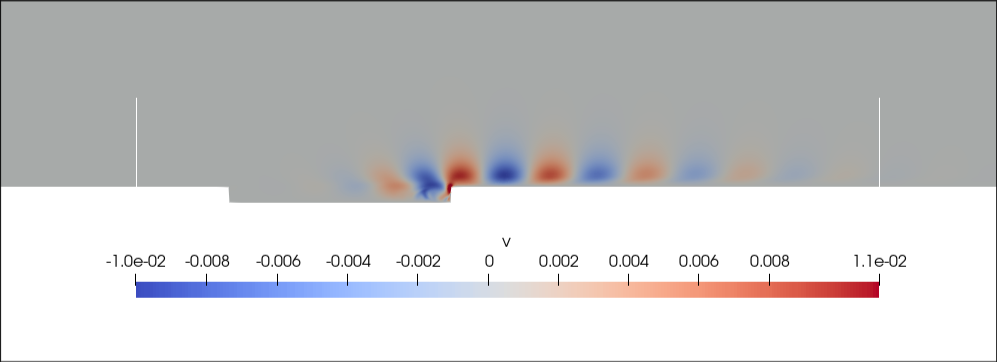
\includegraphics[width=\linewidth]{Images/abs_mode_inside_gap.png}
		\end{column}
		\begin{column}{0.48\linewidth} % Left column
			\centering
			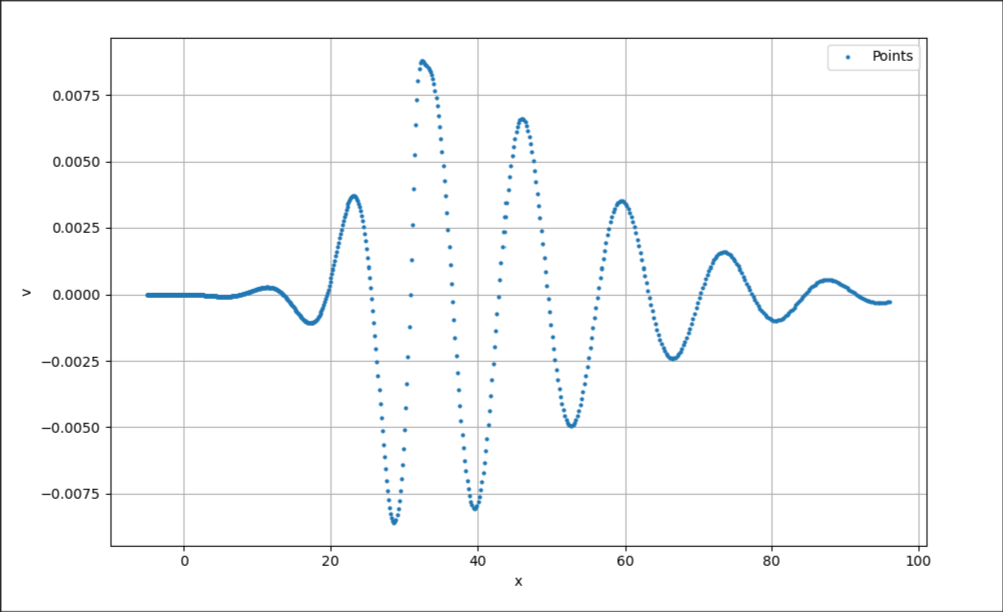
\includegraphics[width=\linewidth]{Images/spatial_evolution_absmode.png}
		\end{column}
	\end{columns}

  
\end{frame}
\begin{frame}
	\frametitle{Frequency comparison in a chaotic regime}
	\begin{itemize}
		\item We study the case $d=3.83$, $w=20$ (see the figure below)
		\item Jeff claims that the dominant nondimensional frequency before transitioning is $F=10^6 \omega \nu /U^2 = 168$
		\item In our case, using that formula we have that $F = 10^3 \omega$ (right? because $U=1$ and $\nu=\frac{1 \times 1}{1000}$).
	\end{itemize}
	\centering
	\small
	\begin{columns}[T] % [T] ensures correct vertical alignment
		\begin{column}{0.245\linewidth} % Left column
			$x=w+5\delta^*$\\
			Dominant freq for \textbf{u}
			$ \omega : 66.428, \widehat{f}(\omega): 784.87$
			$ \omega : 67.377, \widehat{f}(\omega): 539.07$
			$ \omega : 65.479, \widehat{f}(\omega): 224.81$
			$ \omega : 200.234, \widehat{f}(\omega): 204.94$
			$ \omega : 68.326, \widehat{f}(\omega): 202.40$\\
			Dominant freq for \textbf{v}
			$ \omega : 66.428, \widehat{f}(\omega): 100.81$
			$ \omega : 133.806, \widehat{f}(\omega): 73.76$
			$ \omega : 67.377, \widehat{f}(\omega): 68.54$
			$ \omega : 668.080, \widehat{f}(\omega): 62.39$
			$ \omega : 801.886, \widehat{f}(\omega): 56.22$
		\end{column}
		\begin{column}{0.245\linewidth} % Left column
			$x=w+25\delta^*$\\
			Dominant freq for \textbf{u}
			$ \omega : 66.856, \widehat{f}(\omega): 578.61$
			$ \omega : 133.712, \widehat{f}(\omega): 390.67$
			$ \omega : 200.567, \widehat{f}(\omega): 239.15$
			$ \omega : 401.135, \widehat{f}(\omega): 152.63$
			$ \omega : 267.423, \widehat{f}(\omega): 147.29$\\
			Dominant freq for \textbf{v}
			$ \omega : 401.135, \widehat{f}(\omega): 94.62$
			$ \omega : 467.990, \widehat{f}(\omega): 80.02$
			$ \omega : 534.846, \widehat{f}(\omega): 77.23$
			$ \omega : 133.712, \widehat{f}(\omega): 63.12$
			$ \omega : 334.279, \widehat{f}(\omega): 62.55$
		\end{column}
		\begin{column}{0.245\linewidth} % Left column
			$x=w+75\delta^*$\\
			Dominant freq for \textbf{u}
			$ \omega : 133.712, \widehat{f}(\omega): 413.21$
			$ \omega : 66.856, \widehat{f}(\omega): 364.18$
			$ \omega : 267.423, \widehat{f}(\omega): 351.61$
			$ \omega : 200.567, \widehat{f}(\omega): 284.69$
			$ \omega : 334.279, \widehat{f}(\omega): 154.04$\\
			Dominant freq for \textbf{v}
			$ \omega : 267.423, \widehat{f}(\omega): 152.65$
			$ \omega : 133.712, \widehat{f}(\omega): 74.76$
			$ \omega : 334.279, \widehat{f}(\omega): 71.96$
			$ \omega : 200.567, \widehat{f}(\omega): 63.06$
			$ \omega : 467.990, \widehat{f}(\omega): 49.21$
		\end{column}
		\begin{column}{0.245\linewidth} % Left column
			$x=w+175\delta^*$\\
			Dominant freq for \textbf{u}
			$ \omega : 133.917, \widehat{f}(\omega): 279.11$
			$ \omega : 66.490, \widehat{f}(\omega): 195.30$
			$ \omega : 71.173, \widehat{f}(\omega): 158.22$
			$ \omega : 132.981, \widehat{f}(\omega): 149.71$
			$ \omega : 67.427, \widehat{f}(\omega): 148.11$
			Dominant freq for \textbf{v}
			$ \omega : 133.917, \widehat{f}(\omega): 45.03$
			$ \omega : 200.408, \widehat{f}(\omega): 42.09$
			$ \omega : 271.581, \widehat{f}(\omega): 32.03$
			$ \omega : 195.725, \widehat{f}(\omega): 27.78$
			$ \omega : 138.600, \widehat{f}(\omega): 26.89$

		\end{column}
	\end{columns}
	\centering
\end{frame}
\begin{frame}
	\frametitle{Stability curve}
	\centering
	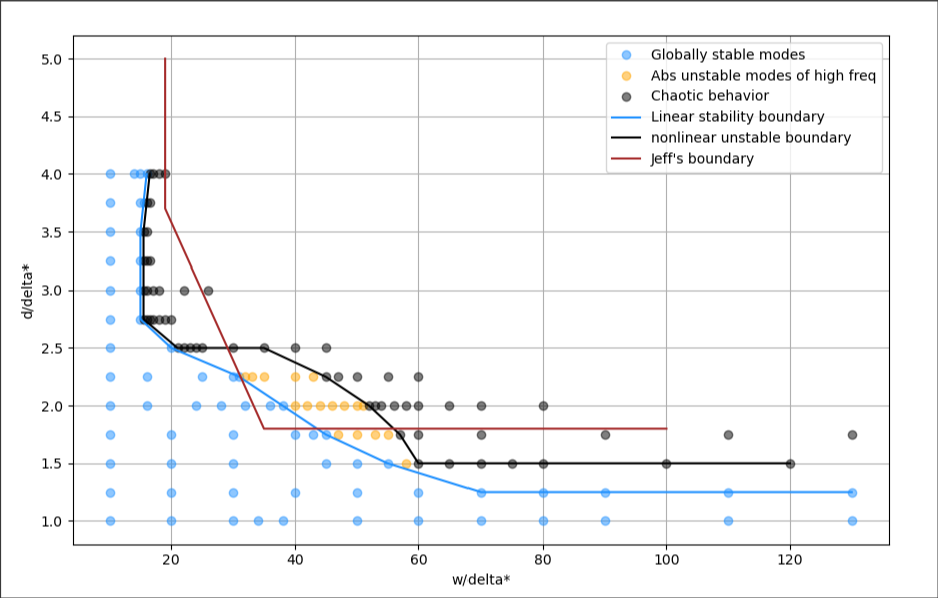
\includegraphics[width=0.75\linewidth]{Images/stabilitycurve.png}
\end{frame}

\begin{frame}
  \frametitle{n-factor computations}

  \centering
  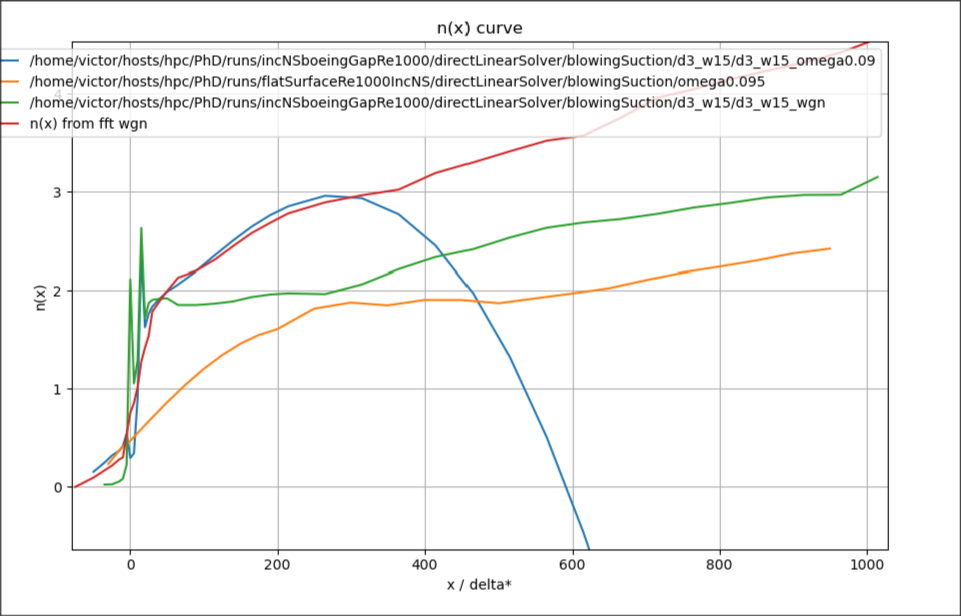
\includegraphics[width=0.75\linewidth]{Images/nfactor.png}
  
\end{frame}
\begin{frame}
  \frametitle{n-factor computations}

  \centering
  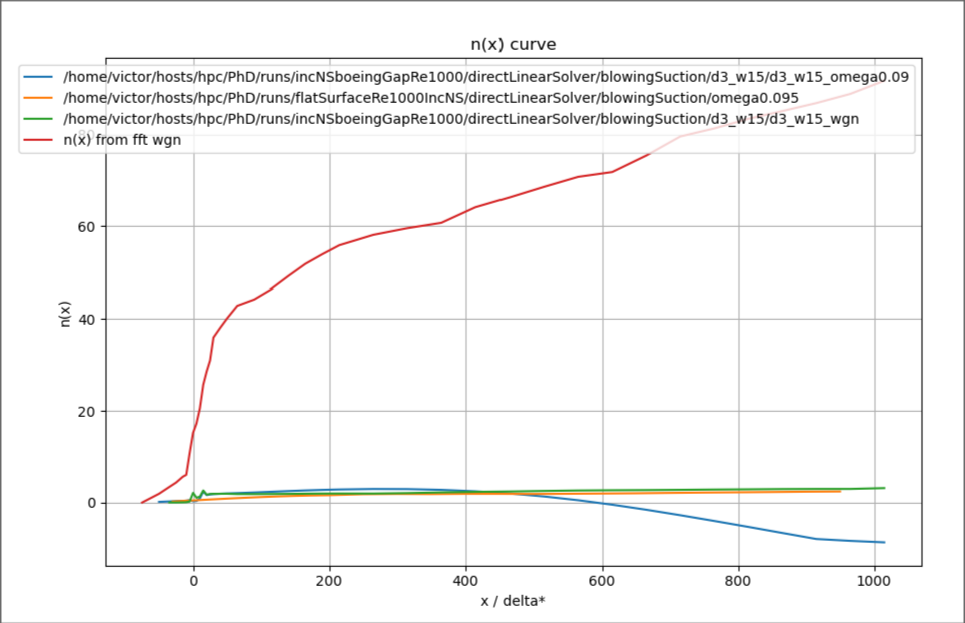
\includegraphics[width=0.75\linewidth]{Images/nfactor_big.png}
  
\end{frame}
\end{document}
